\section{Enriquecimiento de los datos. Aproximación por Vecinos más próximos (K-NN)}
\label{resultados:knn}

\subsection{Características de los conjuntos de datos a analizar}
\label{resultados:knn_caracteristicas}
Una vez realizado todas las transformaciones necesarias para poder ejecutar el algoritmo de \textit{K-NN} podemos observar que tanto el '\textit{Conjunto de datos solo con atributo utilidad definido}' (Caso de estudio 1) como el '\textit{Conjunto de datos sólo con atributo utilidad definido, añadiendo el mes y año del artículo, eliminando los atributos gender y artículo y expandiendo el atributo respuesta.pubmed\_keys}' (Caso de estudio 2) \textbf{se observa el atributo a predecir (utilidad) sesgado}\cite{ref:sesgo} (no tienen un balanceo de datos equilibrado en el atributo a predecir), teniendo más resultados con valor 1 que con valor 0. Esto puede suponer que el modelo resultante tienda a estar sesgado\cite{ref:sesgo} hacia los resultados con valor 1 (debido a que tiene más datos en los que basarse para dar el resultado 1 frente a los otros datos como podemos ver en la figura \ref{knnDistUtilidad}.

\begin{figure}[!htb]
  \centering
    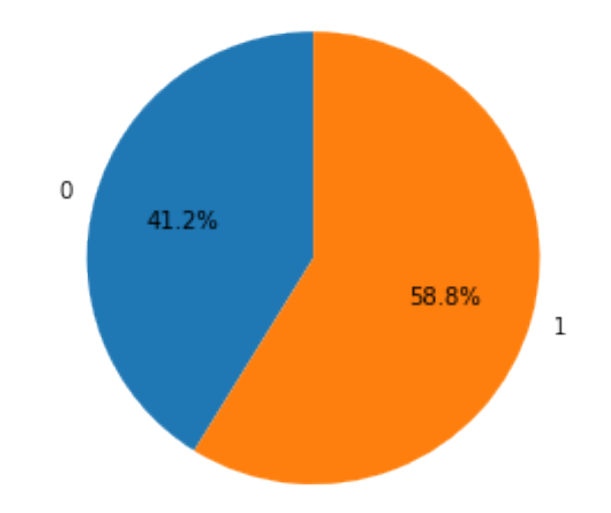
\includegraphics[width=0.3\textwidth]{images/resultados_knn_conjunto1.png}
    \caption{Distribución del atributo a predecir (utilidad) en el conjunto de entrenamiento.}
  \label{knnDistUtilidad}
\end{figure}

También, para el \textbf{caso de estudio 2}, se da el caso que la distribución del \textbf{atributo \textit{pubmed\_keys}}, una vez expandido, también \textbf{se observa sesgado} mostrando algunos resultados con pocas \textit{keywords} y otros como '\textit{Diuresis}' o '\textit{Abdomen}' con muchas observaciones como podemos ver en la figura \ref{knnDistKeywords}. Esto puede condicionar el comportamiento del modelo final igual que en el caso anterior, dando sospechas a que el modelo podría esta sobre ajustado\cite{ref:knn_overfiting}.

\begin{figure}[!htb]
  \centering
    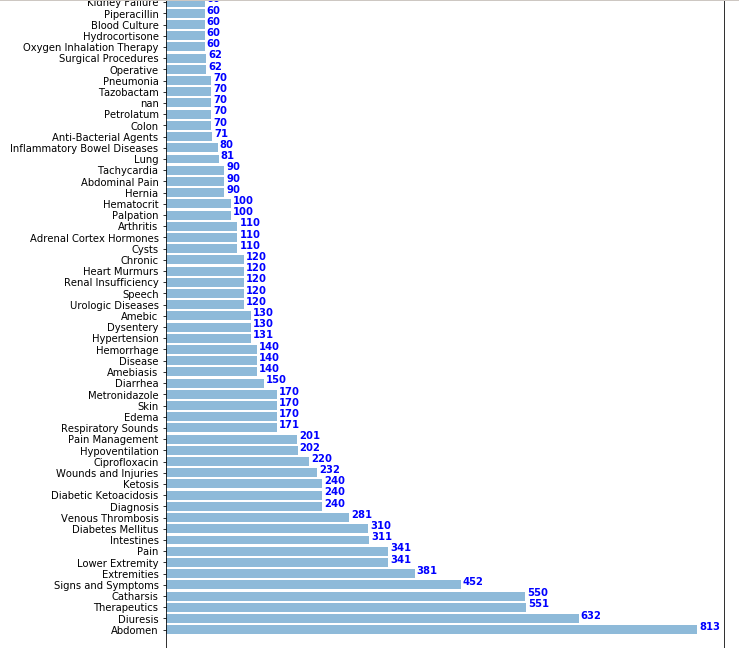
\includegraphics[width=0.8\textwidth]{images/resultados_knn_keywords.png}
    \caption{Distribución del atributo \textit{pubmed\_keys} en el conjunto de entrenamiento.}
  \label{knnDistKeywords}
\end{figure}

\paragraph{}
Finalmente, \textbf{para el entrenamiento y posterior validación} de los modelos nos ayudaremos de la función '\textit{train\_test\_split}'\cite{ref:knn_train_test_split} del paquete '\textit{sklearn\.model\_selection}' que nos permite \textbf{dividir el conjunto de datos en dos grupos}, siendo el \textbf{primer grupo} para realizar el \textbf{entrenamiento} de los modelos que \textbf{corresponde al 75\% del total} de observaciones y el segundo grupo para realizar la \textbf{validación} de los modelos que \textbf{corresponde al 25\% del total} de observaciones.

\subsection{(Caso de estudio 1) Resultados del entrenamiento con el Conjunto de datos solo con atributo utilidad definido}

\paragraph{}
Antes de poder entrenar el algoritmo \textit{K-NN} es necesario realizar un estudio para detectar a partir de que número de vecinos mas próximos (valor K), podemos dar por supuesto que el resultado esta relacionado con ellos. El algoritmo también nos permite poder decidir como calcular la distancia entre los vecinos (bien dando más relevancia a los vecinos con menos distancia '\textit{distance}'\cite{ref:knn_doc} o bien dando la misma relevancia a todos los vecinos que están próximos '\textit{uniform}'\cite{ref:knn_doc}).

Para realizar este estudio ejecutaremos el modelo con diferentes valores de K y contrastaremos que porcentaje de acierto tiene el modelo con un subconjunto del propio conjunto de datos que conocemos su valor final. Como podemos ver en la figura \ref{knnTrainCase1}, el valor más optimo de \textbf{K es 6} utilizando el calculo de la distancia \textbf{'\textit{distance}'}, con un \textbf{porcentaje de acierto del 85\%}.

\paragraph{}
Si mostramos la matriz de confusión\cite{ref:confusion_matrix} (figura \ref{knnCMCase1}) para poder ver que porcentaje de aciertos tiene el modelo con el conjunto de test, vemos que tiene un porcentaje de aciertos bastante aceptable pese a tener más acierto para los casos con resultado 1 vrs. los resultados con valor 0 como comentamos anteriormente.

\begin{figure}[!htb]
    \begin{subfigure}[b]{0.45\linewidth}
    	\centering
	    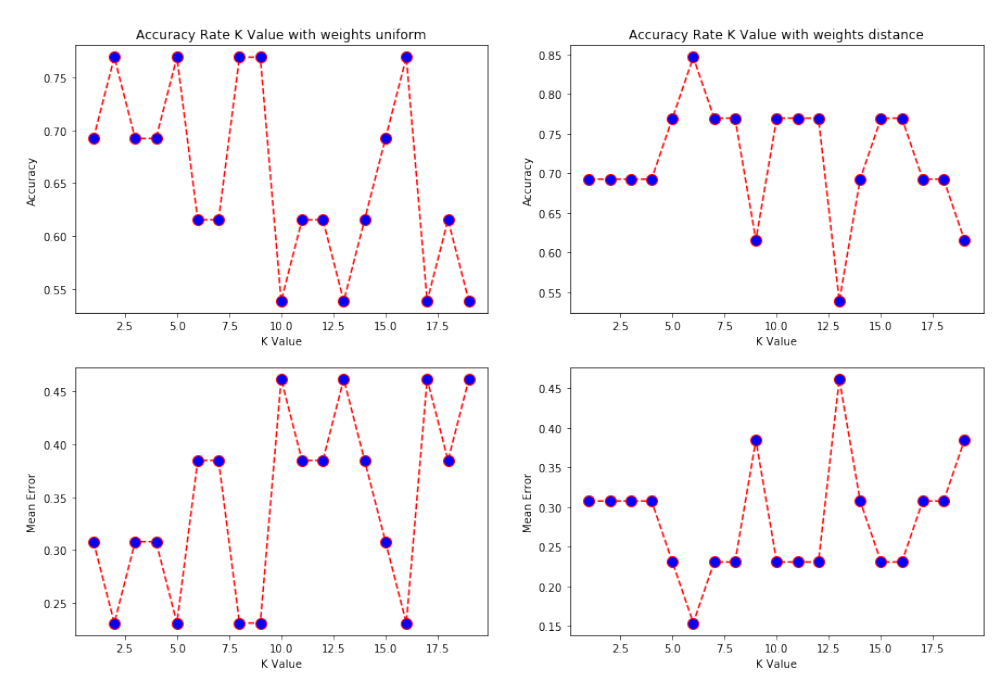
\includegraphics[width=0.9\textwidth]{images/resultados_knn_ent_conjunto1.png}
    	\caption{Calculo del valor K para el caso de estudio 1.}
		\label{knnTrainCase1}
	\end{subfigure}
	\begin{subfigure}[b]{0.45\linewidth} 
		\centering
		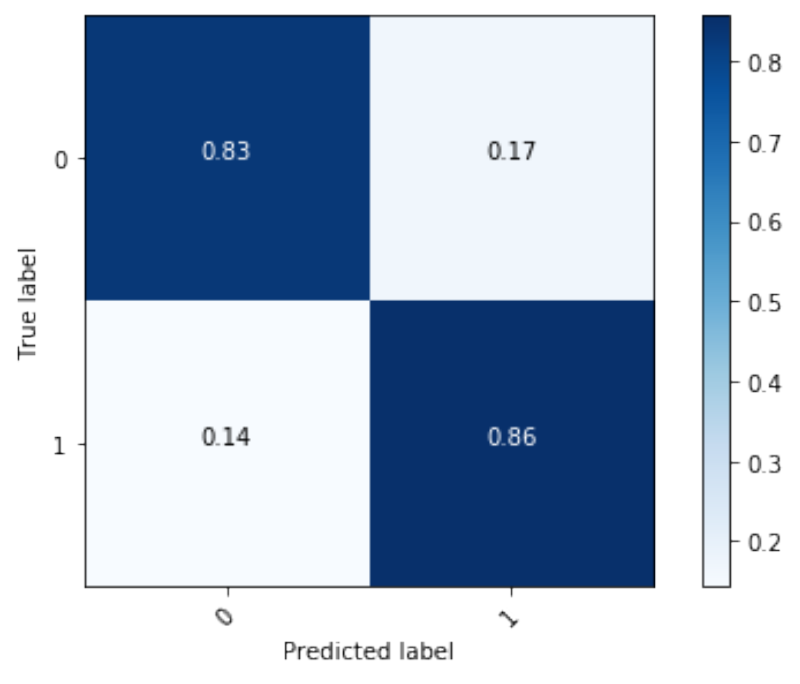
\includegraphics[width=0.7\textwidth]{images/resultados_knn_cm_conjunto1.png}
		\caption{Matriz de confusión para el modelo K-NN en el caso de estudio 1.}
		\label{knnCMCase1}
	\end{subfigure}
	\caption{Modelo K-NN en el caso de estudio 1.}
	\label{knnCase1}
\end{figure}

\subsection{(Caso de estudio 2) Conjunto de datos solo con atributo utilidad definido, añadiendo el mes y año del artículo, eliminando los atributos \textit{gender} y artículo y expandiendo el atributo \textit{respuesta.pubmed\_keys}}

\paragraph{}
Igual que en el caso anterior, realizaremos el estudio para detectar a partir de que número de vecinos mas próximos (valor K), podemos dar por supuesto que el resultado esta relacionado con ellos. A diferencia del caso anterior, podemos ver en la figura \ref{knnTrainCase2}, que el valor más optimo de \textbf{K es 1} utilizando el calculo de la distancia \textbf{'\textit{uniform}'}, con un \textbf{porcentaje de acierto del 90\%}.

Si mostramos la matriz de confusión\cite{ref:confusion_matrix} (figura \ref{knnCMCase2}) para poder ver que porcentaje de aciertos tiene el modelo con el conjunto de test, vemos que tiene un porcentaje de aciertos bastante elevado por lo que podemos afirmar que \textbf{el modelo es sospechoso de estar sobre ajustado\cite{ref:knn_overfiting}}.

\begin{figure}[!htb]
    \begin{subfigure}[b]{0.45\linewidth}
    	\centering
	    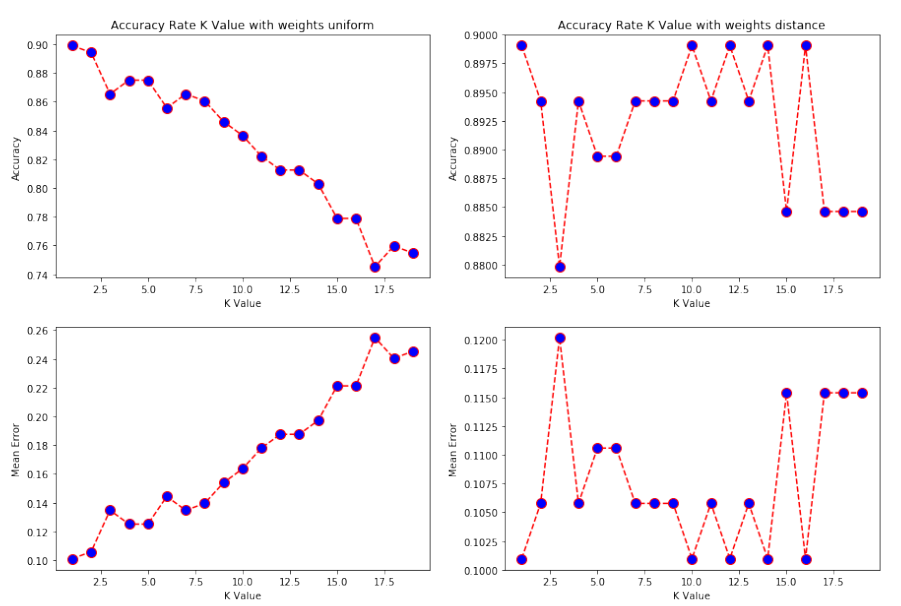
\includegraphics[width=0.9\textwidth]{images/resultados_knn_ent_conjunto2.png}
    	\caption{Calculo del valor K para el caso de estudio 2.}
		\label{knnTrainCase2}
	\end{subfigure}
	\begin{subfigure}[b]{0.45\linewidth} 
		\centering
		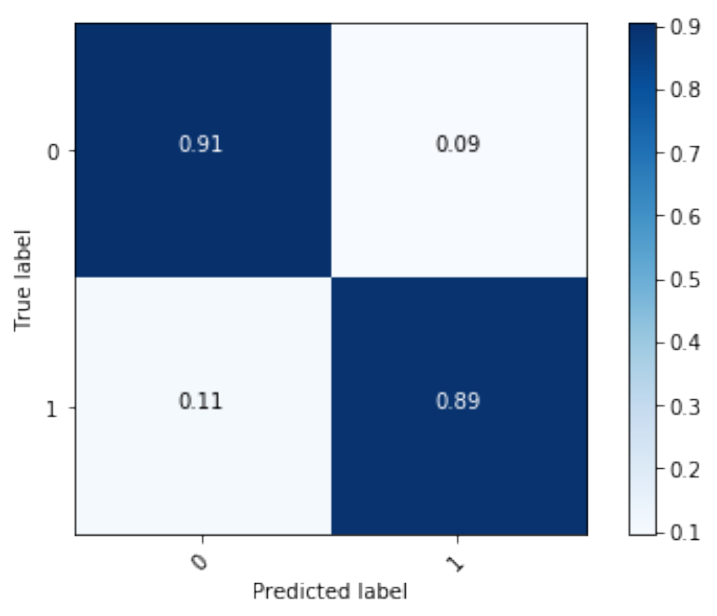
\includegraphics[width=0.7\textwidth]{images/resultados_knn_cm_conjunto2.png}
		\caption{Matriz de confusión para el modelo K-NN en el caso de estudio 2.}
		\label{knnCMCase2}
	\end{subfigure}
	\caption{Modelo K-NN en el caso de estudio 2.}
	\label{knnCase1}
\end{figure}

\subsection{Conclusiones del algoritmo K-NN}
\label{resultados:knn_conclusiones}

\paragraph{}
Pese a que aparentemente, el caso de estudio 1 tiene unos resultados aceptables, \textbf{aconsejamos} al cliente \textbf{no utilizar el algoritmo de \textit{K-NN}} para enriquecer los datos del dataset, prediciendo las observaciones que se desconocen su resultado final. Esto es \textbf{debido} a que detectamos que \textbf{el conjunto de datos se encuentra \hyperref[resultados:knn_caracteristicas]{sesgado}} en varios atributos, lo que hará que el modelo tienda a dar falsos positivos (como hemos podido ver en el caso de estudio 2), perjudicando el entrenamiento de posteriores modelos predictivos que estudiaremos en este documento.